\setchapterstyle{lines}
\chapter[Not Simple Systems Equations]{Not Simple Systems Equations}
\labch{notSimpleSystems}

\renewcommand{\row}[2]{
	\multicolumn{4}{l}{#1} \\
	\multicolumn{2}{>{\centering\arraybackslash}m{4cm}}{\small $#2$} &
}
\renewcommand{\separation}{
			\multicolumn{4}{c}{}\\[-1em]
	        \hline
	        \multicolumn{4}{c}{}\\[-1em]
}

\begin{table}[!h]
	\caption{Transfer functions}
	\labtab{transferFunctions}
	 	\begin{tabular}{>{\centering\arraybackslash}m{2.1cm} | >{\centering\arraybackslash}m{3.15cm} | >{\centering\arraybackslash}m{2.1cm} | >{\centering\arraybackslash}m{3.15cm}}
		        \hline
		        \multicolumn{4}{c}{}\\[-1em]
		        \multicolumn{2}{l}{Gear train} & \multicolumn{2}{l}{Solenoid}Solenoid\\
		        $1$ & 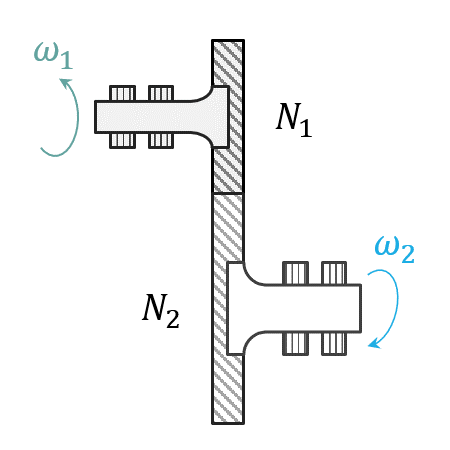
\includegraphics[width=0.02\textwidth]{appendix_notSimpleSystemsEquations/Gear train} & 
		        $2$ & 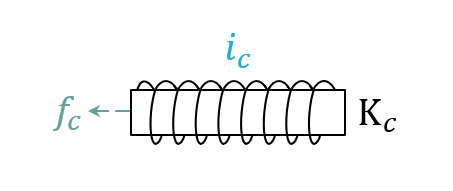
\includegraphics[width=0.02\textwidth]{appendix_notSimpleSystemsEquations/Solenoid}\\
		        \separation
		        \row{Tachometer, velocity sensor}{3} \multicolumn{2}{>{\centering\arraybackslash}m{6.5cm}}{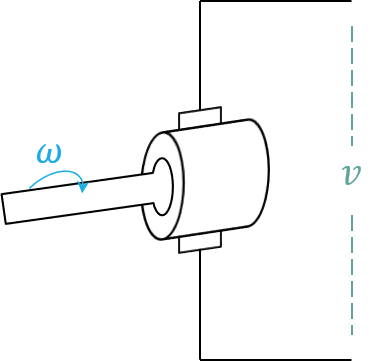
\includegraphics[width=0.1\textwidth]{appendix_notSimpleSystemsEquations/Tachometer}} \\
		        \separation
		        \row{AC motor, two-phase control field}{4} \multicolumn{2}{>{\centering\arraybackslash}m{6.5cm}}{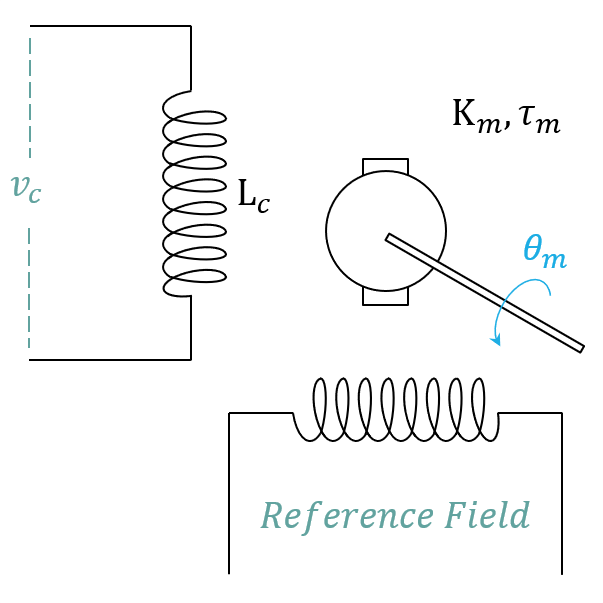
\includegraphics[width=0.1\textwidth]{appendix_notSimpleSystemsEquations/AC motor}} \\
		        \separation
		        \row{Amplidyne, rotary amplifier}{5} \multicolumn{2}{>{\centering\arraybackslash}m{6.5cm}}{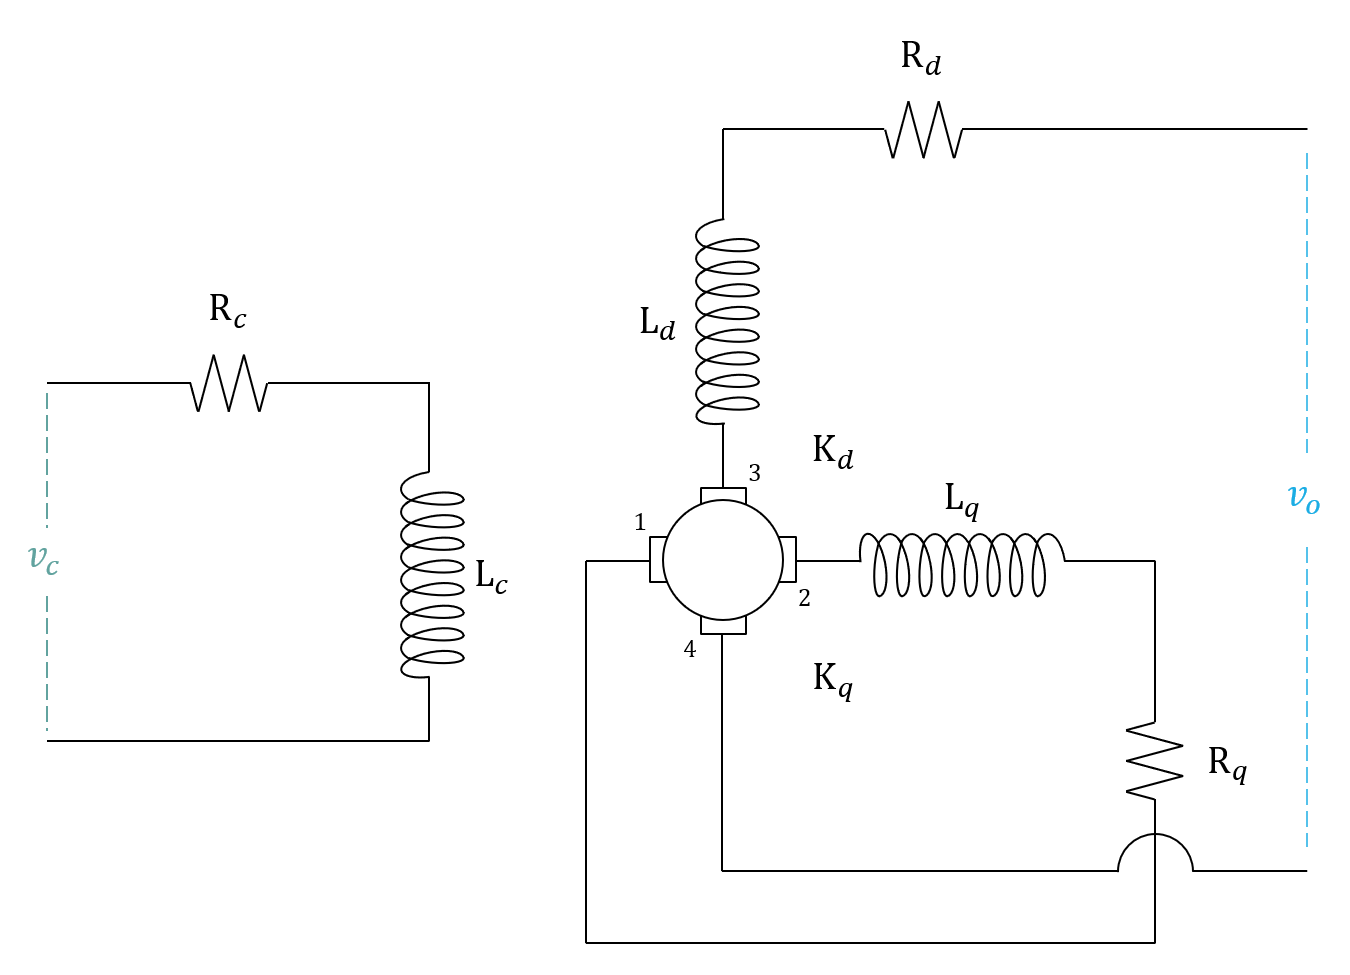
\includegraphics[width=0.1\textwidth]{appendix_notSimpleSystemsEquations/Amplidyne}} \\
		        \separation
		        \row{DC amplifier, 0 Hz amplifier}{6} \multicolumn{2}{>{\centering\arraybackslash}m{6.5cm}}{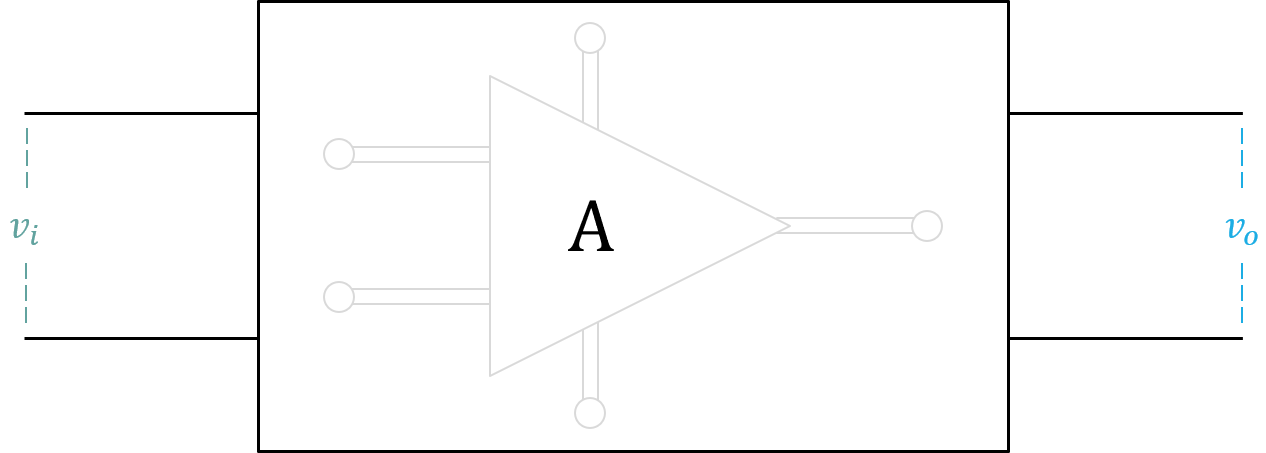
\includegraphics[width=0.1\textwidth]{appendix_notSimpleSystemsEquations/DC amplifier}} \\
		        \separation
		        \row{Demodulator, AC modulated signal to DC}{7} \multicolumn{2}{>{\centering\arraybackslash}m{6.5cm}}{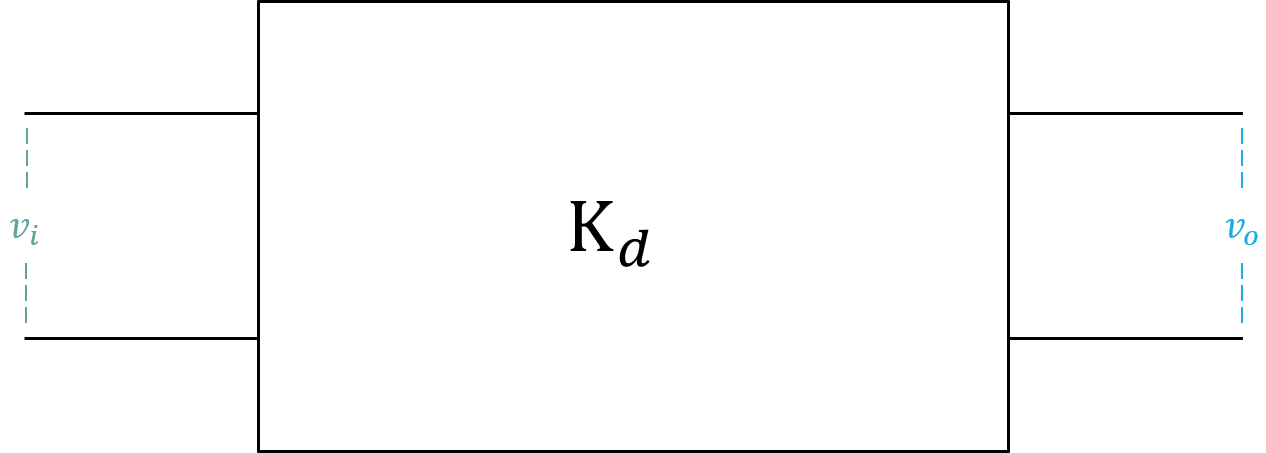
\includegraphics[width=0.1\textwidth]{appendix_notSimpleSystemsEquations/Demodulator}} \\
		        \separation
		        \row{Potentiometer, used in ``Error detector brigde''}{8} \multicolumn{2}{>{\centering\arraybackslash}m{6.5cm}}{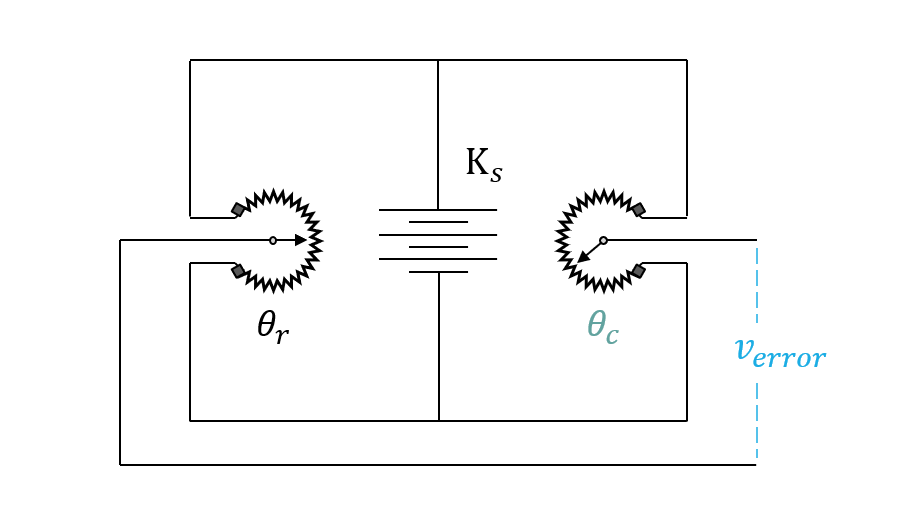
\includegraphics[width=0.1\textwidth]{appendix_notSimpleSystemsEquations/Potentiometer}} \\
		        \separation
		        \row{Synchro, as ``Error detector''}{9} \multicolumn{2}{>{\centering\arraybackslash}m{6.5cm}}{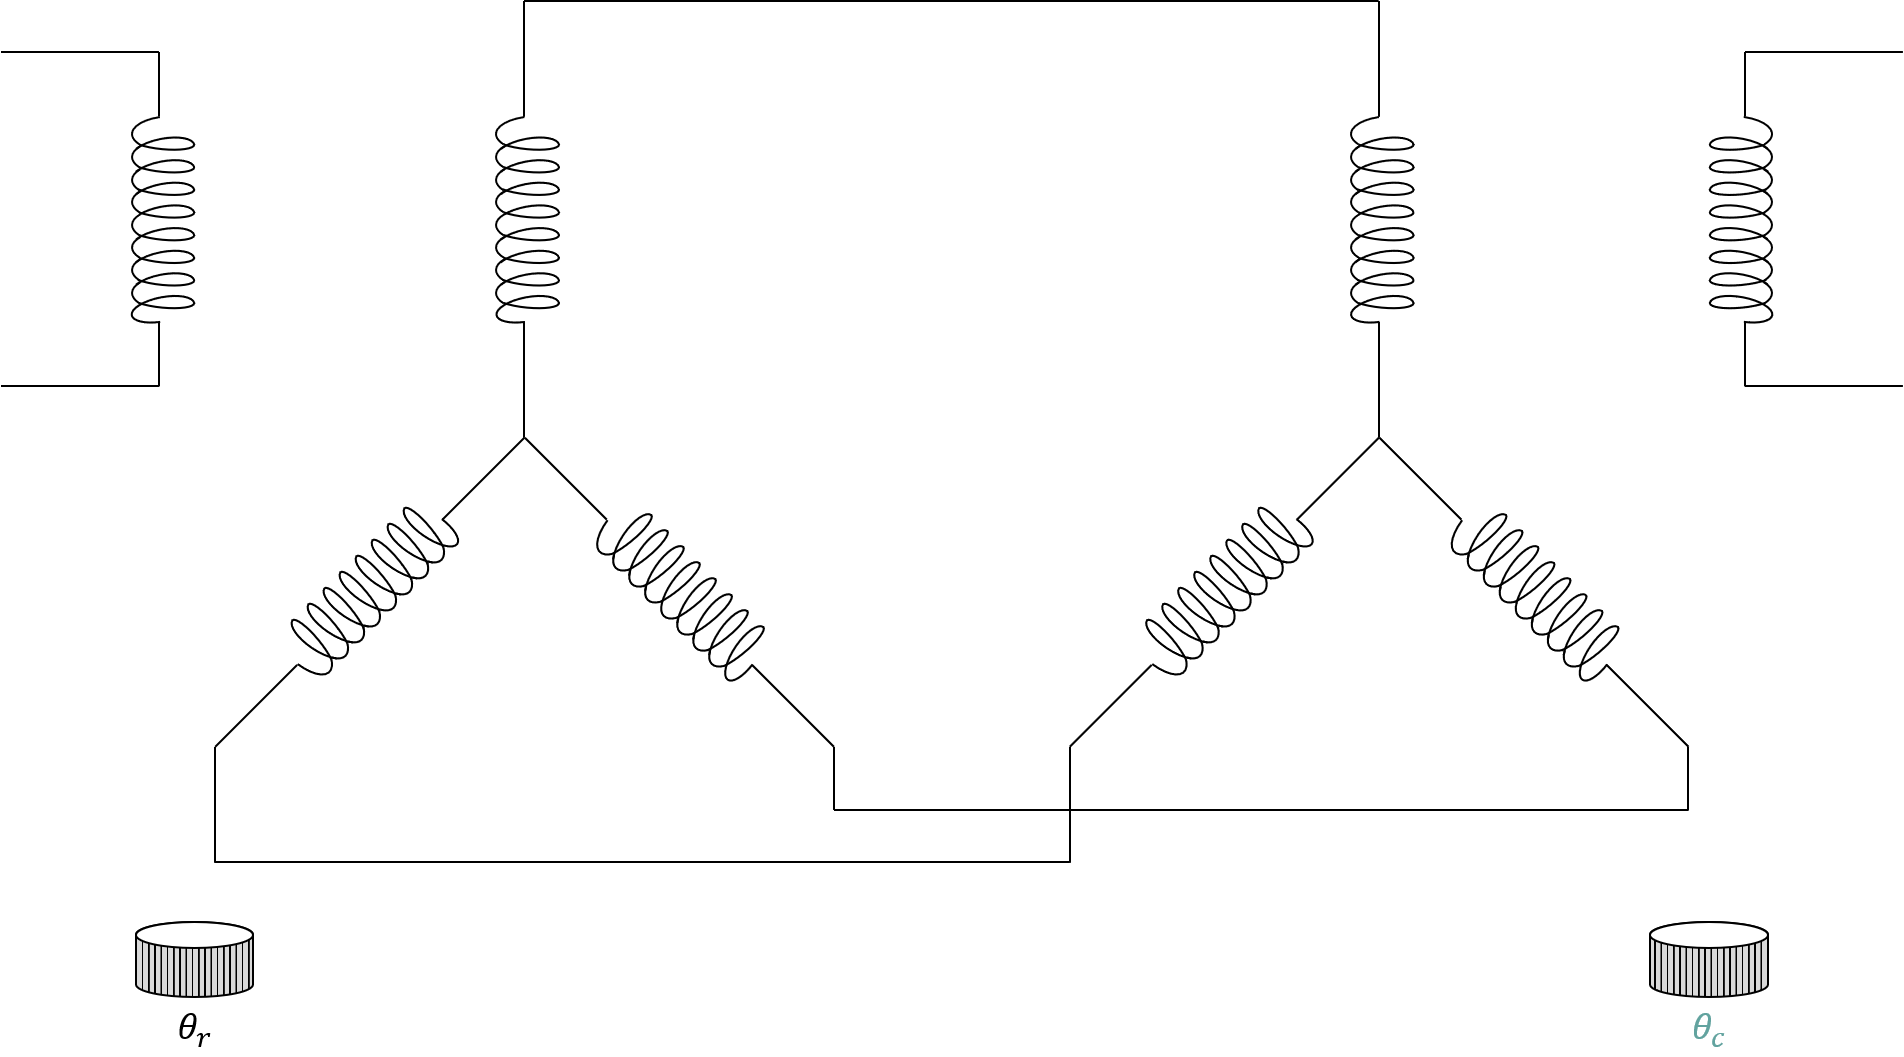
\includegraphics[width=0.1\textwidth]{appendix_notSimpleSystemsEquations/Synchro}} \\
		        \multicolumn{4}{c}{}\\[-1em]
		        \hline
		    \end{tabular}
\end{table}

\begin{description}
\item[Reference] Modern control systems.\footnote{Tables 2-4 ``International Edition''}
			\\\note{Richard c. Dorf, Robert h.Bishop}
\end{description}